% Valentino Vranic
% Metody inzinierskej prace 2012/13

\documentclass{beamer}

%\usetheme{Warsaw}
\usetheme{Antibes}
%\usetheme{JuanLesPins}
%\usetheme{Goettingen}

%\usecolortheme{seahorse}
%\usecolortheme{dolphin}
%\usecolortheme{rose}
% http://deic.uab.es/~iblanes/beamer_gallery/index_by_color.html
\usecolortheme{beaver}

%\useoutertheme[]{sidebar}

\setbeamercovered{transparent}

\usepackage[slovak]{babel}
\usepackage[T1]{fontenc}
\usepackage[utf8]{inputenc}
\usepackage{url}

\usepackage{listings}

\lstset{language=C++,basicstyle=\fontsize{8}{9.6}\selectfont,showstringspaces=false,columns=fullflexible,identifierstyle=\ttfamily,keywordstyle=\bfseries,showstringspaces=false,columns=fullflexible}
%\lstset{language=C,basicstyle=\fontsize{10.5}{12.6}\selectfont,identifierstyle=\ttfamily,keywordstyle=\bfseries,showstringspaces=false,columns=fixed}

\def\BibTeX{\textsc{Bib}\kern-.08em\TeX} 

\newcommand{\footcite}[1]{\footnote{\tiny #1}}
\newcommand{\umlet}{.5}
\newcommand{\emp}[1]{\textit{\alert{#1}}}
\newcommand{\kw}[1]{\mbox{\textbf{#1}}}
\newcommand{\id}[1]{\texttt{#1}}
\newcommand{\stl}{\guillemotleft}
\newcommand{\str}{\guillemotright}

\newcommand{\lsti}{\lstinline[basicstyle=\fontsize{10.5}{12.1}\selectfont]}

\newcommand{\ssection}[1]{
	\section{#1}
	\begin{frame}[fragile=singleslide]\frametitle{}
	\Huge #1
	\end{frame}
}

\newcommand{\ssectionn}[1]{
	\section*{#1}
	\begin{frame}[fragile=singleslide]\frametitle{}
	\Huge #1
	\end{frame}
}

\newenvironment{program}{\begin{beamercolorbox}[rounded=true,shadow=true]{block body}\vspace{-4mm}}{\vspace{-2mm}\end{beamercolorbox}}

\setbeamercolor{fvystup}{fg=white,bg=black}
\newenvironment{vystup}{\begin{beamercolorbox}[rounded=true,shadow=true]{fvystup}}{\end{beamercolorbox}}

\newenvironment{poznamka}{\begin{beamercolorbox}[rounded=true,shadow=false]{block body}}{\end{beamercolorbox}}

\setbeamertemplate{footline}[page number]
{
%\insertpagenumber
%\begin{beamercolorbox}{section in head/foot}
%\vskip2pt\insertnavigation{\paperwidth}\vskip2pt
%\end{beamercolorbox}%
}



\author{Branislav Trstenský}
%\url{www.fiit.stuba.sk/~vranic}, \url{vranic@fiit.stuba.sk}}
%{\tiny \url{www.fiit.stuba.sk/~vranic}, \url{vranic@fiit.stuba.sk}}
\institute{
	Ústav informatiky, informačných systémov a softvérového inžinierstva\\
	Fakulta informatiky a informačných technológií\\
	Slovenská technická univerzita v Bratislave}

\subtitle{\vspace{3mm} Metódy inžinierskej práce 2022/2023}

\title{Gamifikácia pre učenie cudzích jazykov
}

\date{\footnotesize 9. november 2022}




\begin{document}

\begin{frame}[fragile=singleslide,plain]
\titlepage
\end{frame}


\begin{frame}[fragile=singleslide,plain]\frametitle{Prečo gamifikácia}
\begin{itemize}
\item Zvýšená potreba znalosti cudzích jazykov
\item Učenie jazykov je namáhavé
\item Gamifikácia: zdroj motivácie, udržiava pravidelné štúdium
\end{itemize}
\end{frame}


\begin{frame}[fragile=singleslide,plain]\frametitle{Prehľad}
\tableofcontents
\end{frame}


\section{Gamifikácia všeobecne}
% príkaz \ssection by vytvoril zvláštný slajd s názvom časti - v krátkych prezentáciách to prekáža, lebo oberá o čas

\begin{frame}[fragile=singleslide,plain]\frametitle{Gamifikácia všeobecne}
\begin{itemize}
\item Hry umožňujú rozvíjanie kognitívnych schopností
\item Proces učenia prebieha intuitívne a spontánne počas hrania
\item Tréning schopností je výsledkom zapájania sa do úloh, ktoré hra vyžaduje
\item Neustále opakovanie v rámci hernej slučky
\item Motivovácia odmenami, alebo pocitom prekonania výziev
\end{itemize}
\end{frame}

\section{Prvky gamifikácie}

\begin{frame}[fragile=singleslide,plain]\frametitle{Prvky gamifikácie}
\begin{center}
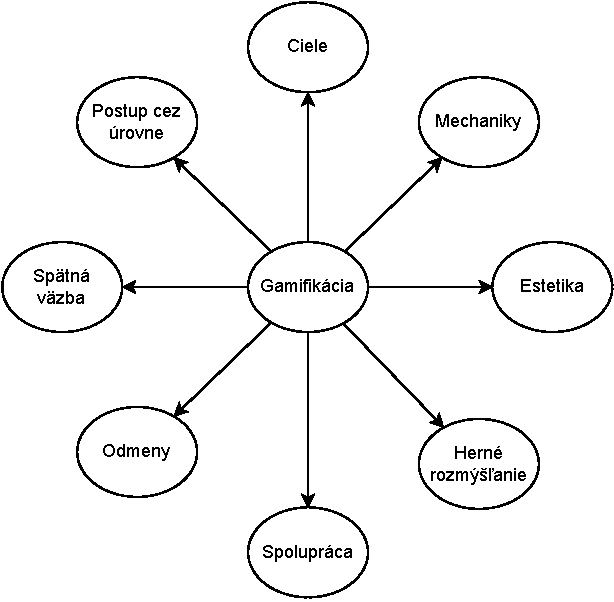
\includegraphics[scale=.6]{prvky.pdf}
% pridajte vlastný obrázok a zrušte znák % pred príkazom \includegraphics vo formáte PDF prípadne PNG alebo JPG
% scale určuje veľkosť obrázku

{\tiny Prvky Gamifikácie}
\end{center}
\end{frame}


\begin{frame}[fragile=singleslide,plain]\frametitle{Prvky gamifikácie}
\begin{itemize}
\item Ciele
	\begin{itemize}
	\item Sústredenie na učenie
	\item Prechodné ciele
	\end{itemize}
\item Mechaniky
	\begin{itemize}
	\item Pravidlá, určujú priebeh hry
	\item Štruktúra, funkcionalita
	\item Riadia proces učenia
	\end{itemize}
\item Esteticka
	\begin{itemize}
	\item Udržanie záujmu hráča
	\item Prostredie, ktoré hráča ponorí do hry
	\end{itemize}
\item Herné rozmýšľanie
	\begin{itemize}
	\item Premena tradičných učebných aktivít
	\item Z výučbových situácií vytvoriť herné systémy
	\end{itemize}
\end{itemize}
\end{frame}
\begin{frame}[fragile=singleslide,plain]\frametitle{Prvky gamifikácie}
\begin{itemize}
\item Spolupráca
	\begin{itemize}
	\item Zlepšuje účinnosť
	\item Výmenu skúseností a vzájomnú pomoc medzi študentmi
	\end{itemize}
\item Odmeny
	\begin{itemize}
	\item Dôležité pre motiváciu
	\item Zlepšené v sociálnom kontexte
	\end{itemize}
\item Spätná väzba
	\begin{itemize}
	\item Konštantne k dispozícií
	\item Ukazuje študentovi stupeň úspešnosti
	\item Pomáha k lepšiemu výkonu
	\end{itemize}
\item Postup cez úrovne
	\begin{itemize}
	\item Udržiava pozornosť hráča
	\item Zvýšenie náročností úloh
	\item Pocit prekonania výzvy
	\end{itemize}
\end{itemize}
\end{frame}

\section{Gamifikácia výučby jazyka v praxi}

\begin{frame}[fragile=singleslide,plain]\frametitle{Gamifikácia výučby jazyka v praxi}
\begin{center}
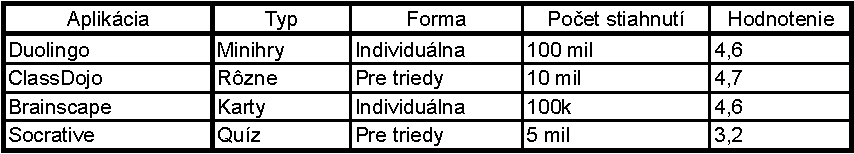
\includegraphics[scale=.7]{aplikacie.pdf}

{\tiny Aplikácie využívajúce gamifikáciu}
\end{center}
\end{frame}



\section*{Zhodnotenie}
% hviezdička zabezpečí, aby sa táto časť neocitla v prehľade prezentácie - každá prezentácia má zhodnotenie a prehľad by sa tým zbytočne zahlcoval

\begin{frame}[fragile=singleslide,plain]\frametitle{Zhodnotenie}
\begin{itemize}
\item Gamifikácie pomáha pri výučbe jazyka
\item Aktívne použítie v praxy
\item Popularita dokazuje efektivitu
\end{itemize}
\end{frame}


\end{document}

